\chapter{METHODOLOGY}
\section{System Development Approach}
An incremental approach, also known as an iterative or step-by-step approach, is a development or problem-solving method that breaks down a larger task or project into smaller, manageable increments or steps. Rather than attempting to tackle the entire task at once, an incremental approach focuses on making incremental progress by completing and delivering smaller portions of work in a series of iterations.
\begin{itemize}
    \setlength\itemsep{0.25em}
    \item Initial Planning and Requirements Gathering
    \item Increment Planning and Design
    \item Development and Implementation
    \item Testing and Quality Assurance
    \item Evaluation and Feedback
    \item Iterative Development and Refinement
    \item Deployment and Release
    \item Repeat the Process for Subsequent Increments
\end{itemize}
\section{Requirement Analysis}
\subsection{Functional Requirements}
The functional requirements of LabXplorer are mentioned below:
\begin{itemize}
    \item \textbf{User Profiles and Progress Tracking:} LabXplorer allows children and teachers to create personalized profiles to track their progress and achievements. Users can log in with unique credentials, update profiles with educational interests and avatars, and monitor completion of experiments and simulations. Progress tracking includes recording tasks completed, concepts learned, and unlocking achievements, providing a comprehensive overview of individual learning journeys.
    \item \textbf{Interactive Virtual Laboratories:} LabXplorer features interactive virtual labs including Basic Electronics, Basic Chemistry, Basic Astronomy, and an online Coding Environment. These labs offer immersive simulations where users engage in hands-on activities like experiments and equipment manipulation. Through interactive animations and real-world scenarios, LabXplorer facilitates experiential learning, enabling exploration of scientific principles and phenomena in a dynamic digital environment.
    \item \textbf{Teacher Tools and Student Assignments:} Teachers access specialized tools to create experiment workflows and assign tasks to students. Experiment workflows can be customized with sequential steps, interactive assessments, and checkpoints to monitor student progress. Teachers review completed tasks, provide feedback, and assess learning outcomes, fostering personalized learning experiences aligned with educational objectives and curriculum requirements.
    \item \textbf{Discussion Forum for Learning Community:} LabXplorer incorporates a discussion forum where users engage in collaborative learning and knowledge-sharing. Children and teachers initiate discussions, pose questions, share insights, and respond to peers' inquiries. The forum supports threaded discussions, tagging, and search features to facilitate meaningful interactions and peer-to-peer engagement. 
    \item \textbf{Sandbox Mode for Creating Own Experiments:} LabXplorer includes a sandbox mode that allows users to create their own experiments. In this mode, students and teachers can design and conduct custom experiments using virtual tools and resources available in the platform. The sandbox environment supports creativity and exploration, enabling users to test hypotheses, simulate scenarios, and explore scientific concepts beyond predefined lab activities. 
\end{itemize}
\newpage
\subsection{Nonfunctional Requirements}
The nonfunctional requirements of LabXplorer are mentioned below:
\begin{itemize}
    \item \textbf{Performance Enhancement:} The focus on performance involves optimizing the platform to handle high user loads and complex simulations efficiently. This includes minimizing reliance on external frameworks and ensuring smooth and responsive interactions.
    \item \textbf{Authentication Security:} Security is a paramount concern. To enhance the platform’s security, advanced authentication algorithms, particularly focusing on hashing techniques within the backend environment, have been implemented. This ensures that user authentication data is stored and managed in a highly secure manner.
    \item \textbf{Better UX Design:} User experience is central to the project’s success. The emphasis on better UX design means that every aspect of the platform’s interface, from navigation to interaction, will be meticulously crafted to ensure a seamless and intuitive experience. This design approach caters not only to experienced users but also to newcomers, ensuring that all users can effortlessly navigate and engage with the platform.
    \item \textbf{Responsive Design:} Recognizing the diverse range of devices and browsers that users utilize, the creation of a responsive design is important for this project. This means that the platform’s design and functionality will adapt flawlessly to various screen sizes, ensuring that users can access and interact with the platform effectively, whether they are using a desktop computer, tablet, or smartphone. This responsiveness guarantees a consistent and satisfying experience across different devices and platforms, promoting accessibility and usability.
\end{itemize}
\section{Feasibility Analysis}
A feasibility study is a systematic and structured analysis conducted to determine the viability and practicality of a proposed project plan. It serves as an evaluation tool to assess whether the project can be successfully implemented and if it aligns with the organization's goals and objectives. It involves gathering and analyzing relevant information to determine if the project is technically feasible, operationally feasible, economically feasible, and scheduling feasible.
\subsection{Economical Feasibility}
Since the proposed system has a web application, we will be using free and open-source software development tools such as Flutter, Express, Postgres SQL. We will only need some economy for server for hosting.
\subsection{Operational Feasibility}
LabXplorer emphasizes operational feasibility through its user-centric approach, focusing on intuitive design and ease of use. The system is crafted to be highly interactive, allowing users, including students and educators, to navigate effortlessly without requiring extensive mobile app expertise. The user interface (UI) is designed with a clean layout and intuitive controls, ensuring a seamless experience for exploring features such as virtual experiments and educational resources. By minimizing training requirements and reducing potential user resistance, LabXplorer aims to enhance user acceptance and engagement. Overall, its intuitive design facilitates efficient utilization of the app's functionalities, supporting educational activities and fostering a positive user experience 
\subsection{Technical Feasibility}
Combining Express.js with Flutter and PostgreSQL presents a technically feasible approach for developing a modern and scalable application. Express.js, built on Node.js, serves as a powerful backend framework ideal for creating RESTful APIs and managing server-side logic efficiently. PostgreSQL, known for its reliability and advanced features in data management, provides a robust foundation for storing and querying data securely. On the frontend, Flutter offers a unified framework for building responsive and visually appealing applications across multiple platforms using a single codebase. This combination leverages the strengths of each technology: Express.js for backend scalability and API development, PostgreSQL for robust data handling, and Flutter for seamless cross-platform UI development. Supported by active communities and extensive documentation, this stack ensures technical support, resources, and flexibility for deployment and maintenance, making it well-suited for delivering modern, interactive applications.
\section{High Level Design of System}
\subsection{Architecture Design}
The following diagram shows diagram of our Architecture. Mainly shows what are the functions can be accessed after starting our application.
\begin{figure}[H]
    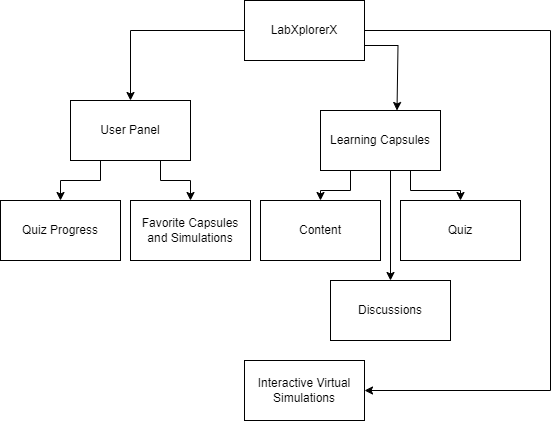
\includegraphics[height = 5.7cm]{Diagrams/Main_Block.png}
    \caption{Main Architecture of System}
\end{figure}
\newpage
\subsection{Data Modelling(ER-Diagram)}
ER Diagram is mainly used to design database schema. With the help of below er diagram we can easily design database in SQL.
\begin{figure}[H]
    \rotatebox{90}{
    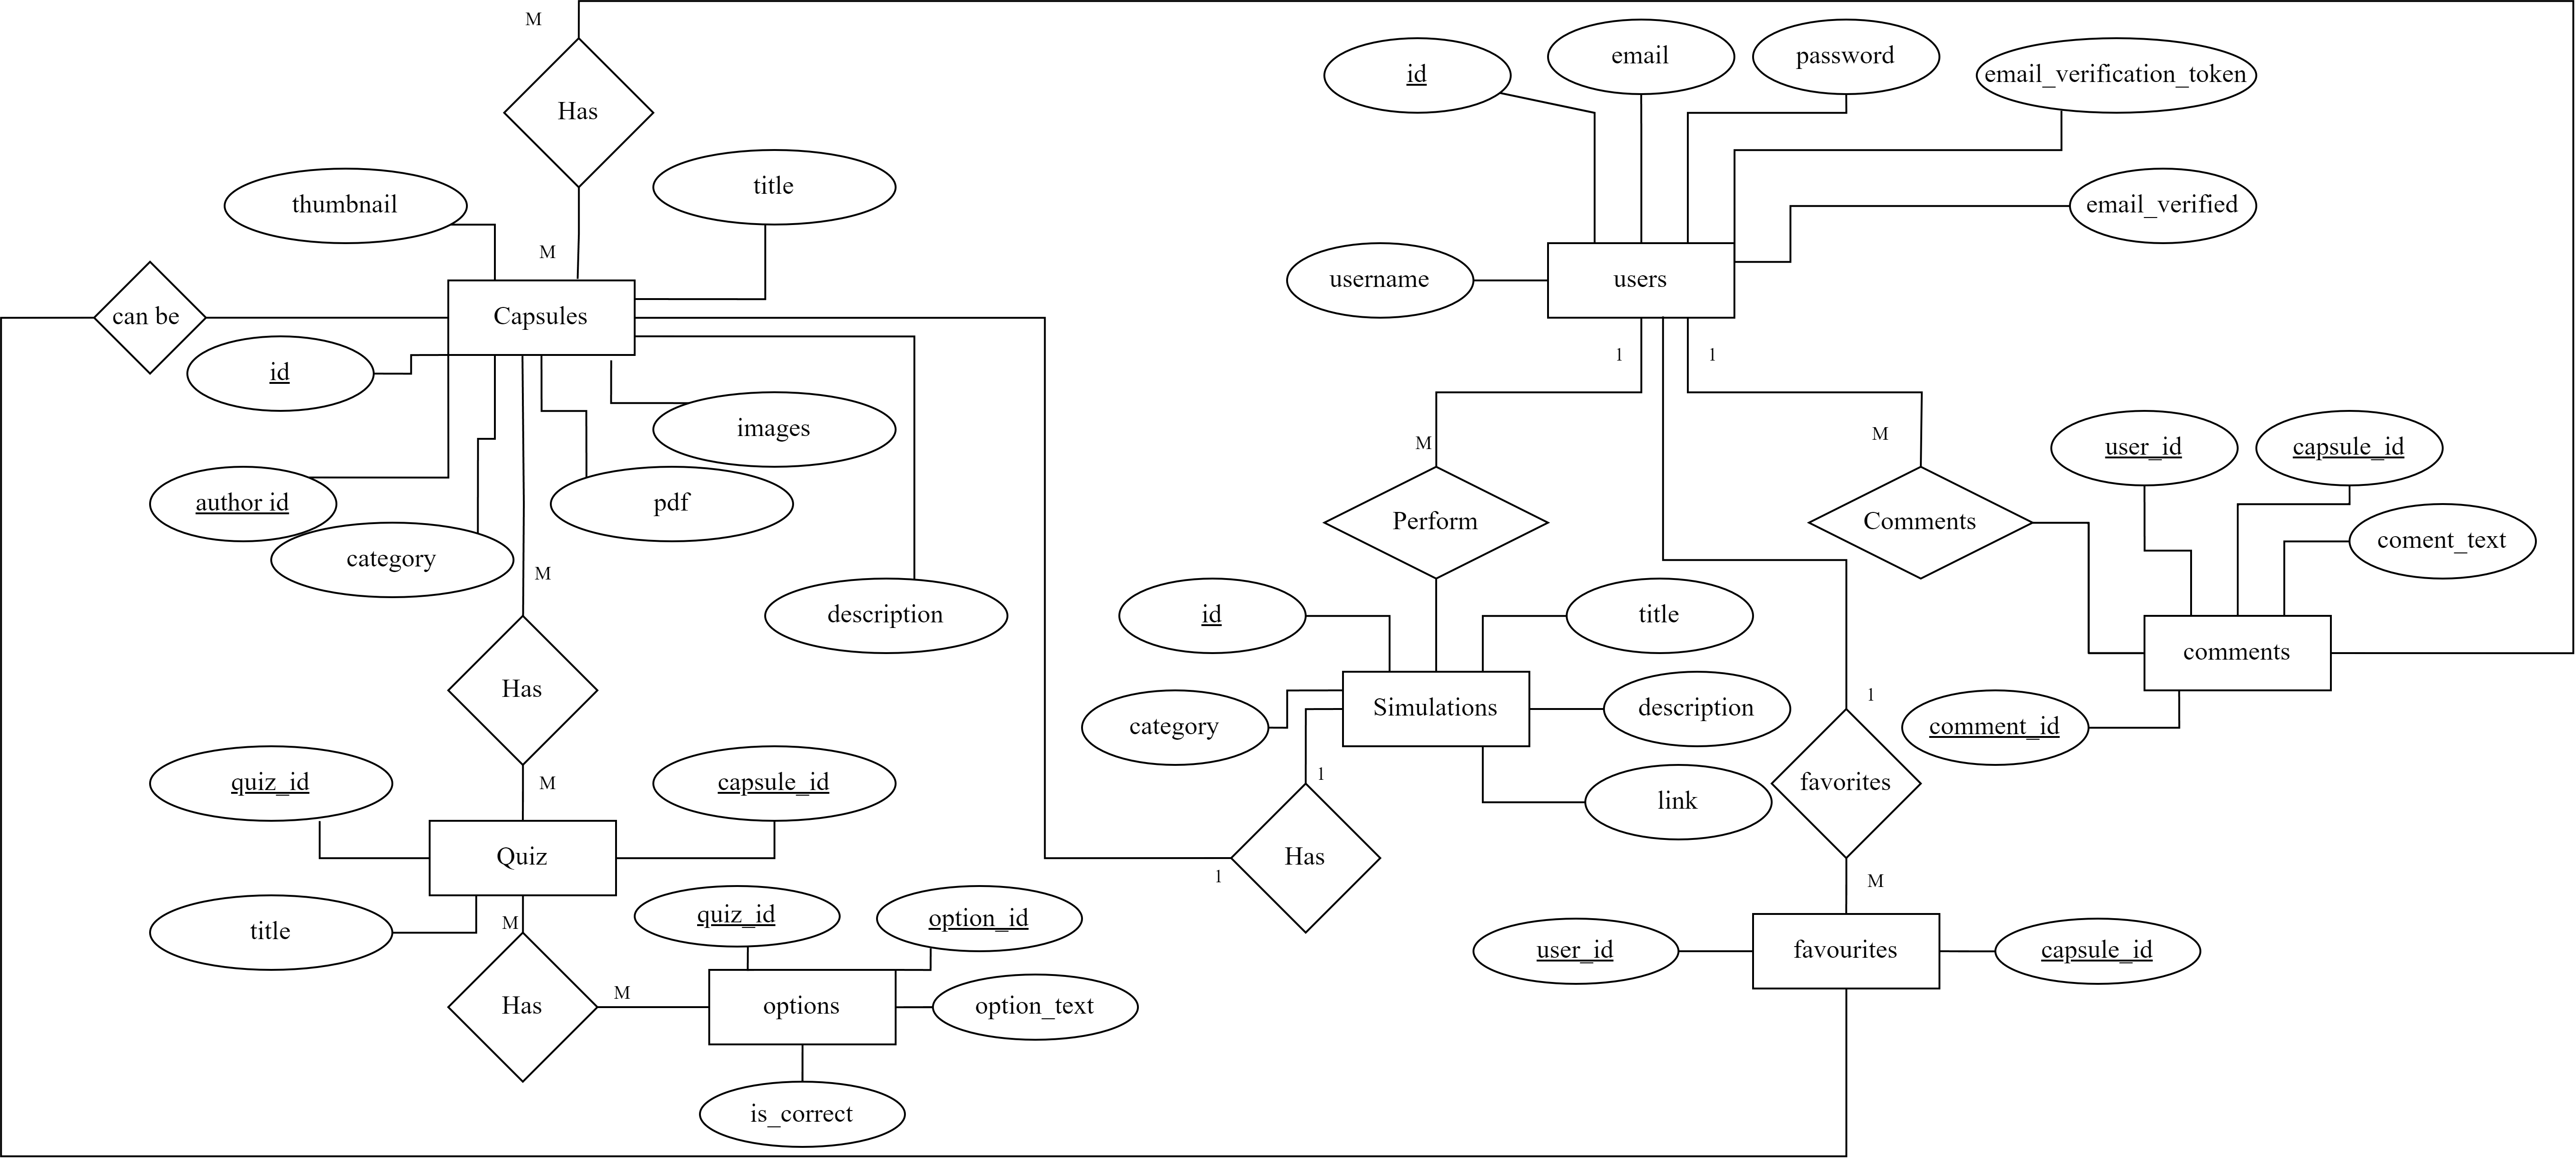
\includegraphics[height = 14cm]{Diagrams/er.drawio.png}}
    \caption{ER Diagram of System Data}
\end{figure}
\newpage
\subsection{Activity Diagram}
An activity diagram visually presents a series of actions or flow of control in a system similar to a flowchart or a data flow diagram. This diagram showed how our program flow goes on.
\begin{figure}[H]
   \centering
    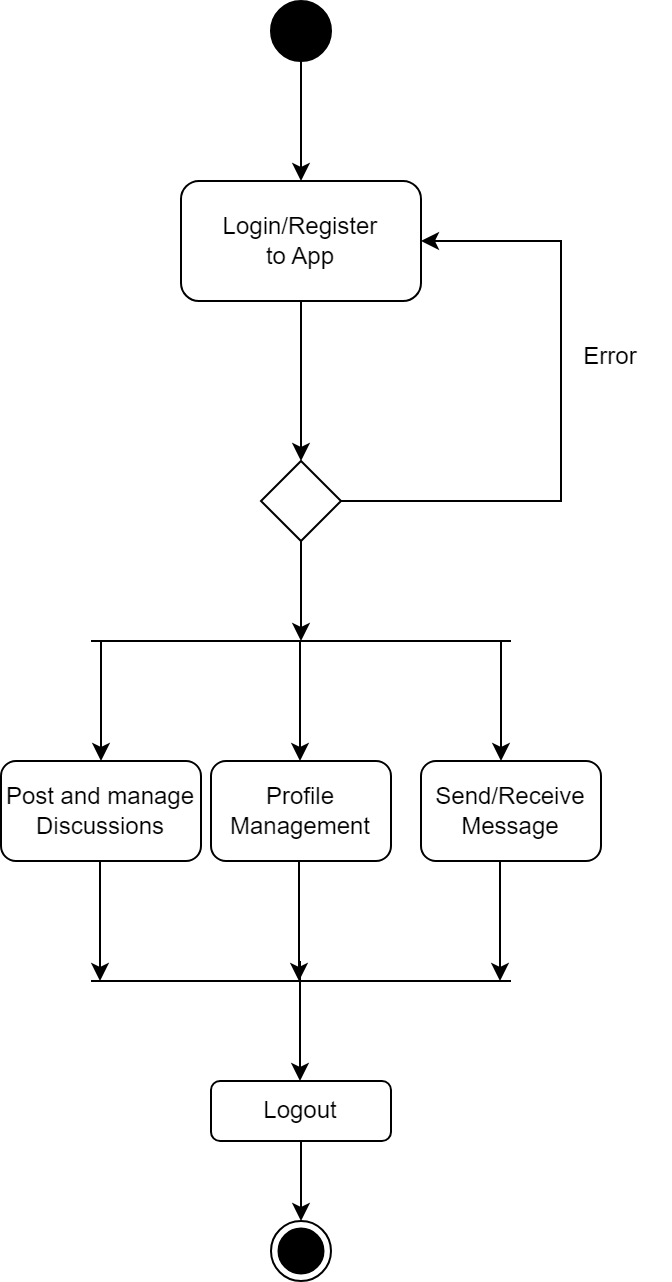
\includegraphics[height = 15cm]{Diagrams/Activity.drawio.png}
    \caption{Activity Diagram}
\end{figure}
\newpage
\subsection{DFD}
DFD or Data Flow Diagram is mainly used to show how data are being flowed in and out of our system. There are 3 levels of DFD i.e Context Level(Level 0),Level 1 and Level 2
\begin{figure}[H]
    \centering
    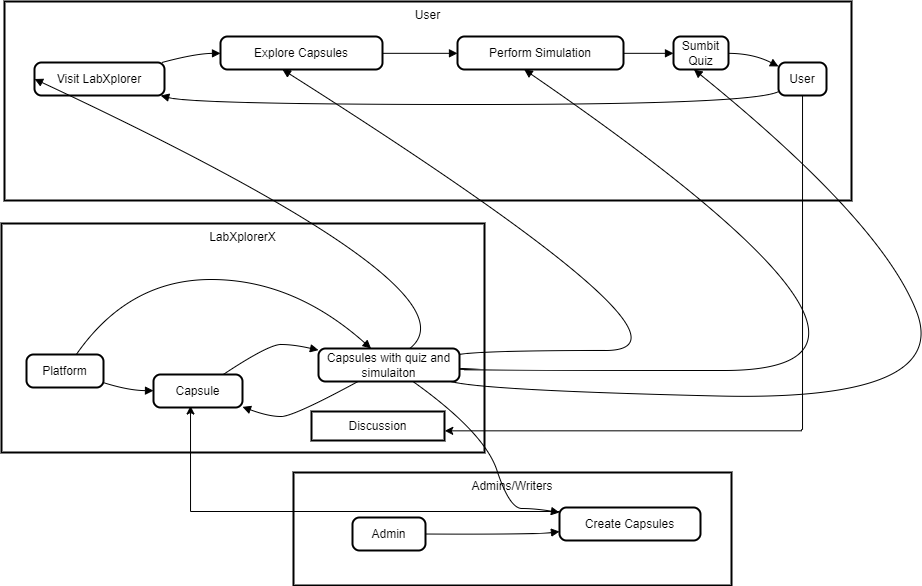
\includegraphics[height = 9cm]{Diagrams/DFD.drawio.png}
    \caption{Data Flow Diagram (Context Level)}
\end{figure}
\newpage
% \subsection{Use Case Diagram}
% A use case diagram, part of UML, visually represents interactions between actors and a system. Actors are external entities, while use cases depict specific functionalities. Relationships, such as association, generalization, include, and extend, illustrate connections between actors and use cases. The diagram helps in understanding system behavior, requirements, and scope.
% \begin{figure}[H]
%     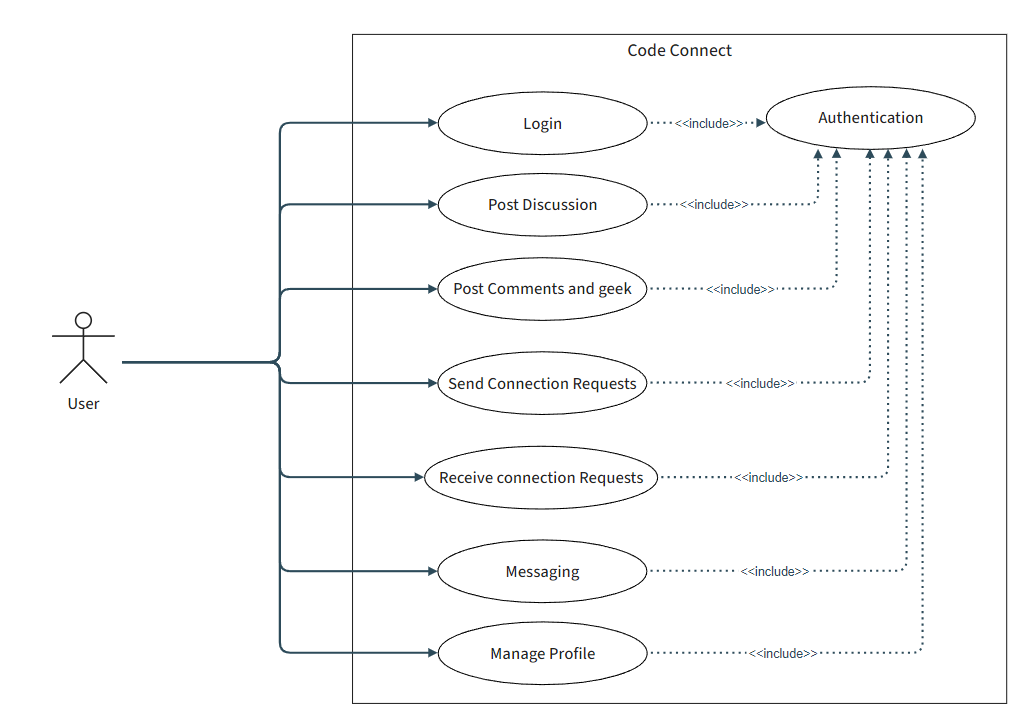
\includegraphics[height = 10cm]{Diagrams/use_case.png}
%     \caption{Use Case Diagram}
% \end{figure}
